\documentclass[border=2pt]{standalone}
\usepackage{tikz}
\usepackage{amsmath}
\usepackage{mathtools}
\usepackage{adjustbox}
\usetikzlibrary{patterns}
\usetikzlibrary{calc} \usetikzlibrary{positioning} \usetikzlibrary{shapes,arrows} \usetikzlibrary{plotmarks}
\usetikzlibrary{positioning,decorations.pathreplacing}
\tikzset{
itria/.style={
  draw,dashed,shape border uses incircle,
  isosceles triangle,shape border rotate=90,yshift=-0.8cm}
}

\begin{document}

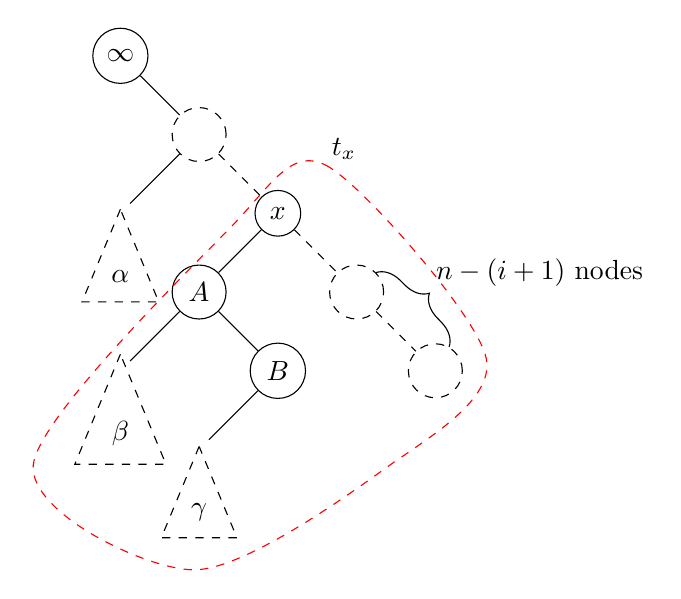
\begin{tikzpicture}[level/.style={sibling distance=20mm, level distance=10mm}]
\node [circle,draw](inf){$\infty$}
  child[missing]{}
  child { node[circle,draw, dashed]{$\phantom{A}$}
    child { node[]{}
            { node[itria]{$\alpha$} }
    }
    child[dashed] { node[circle, draw, solid](Xnode){$x$}
      child[solid] { node[circle, draw, solid](Anode){$A$}
        child[solid] { node[]{}
              { node[itria](BETAnode){$\beta$} }
        }
        child[solid] { node[circle, draw]{$B$}
          child[]{node[]{}
              { node[itria](GAMMAnode){$\gamma$} }
          }
          child[missing]{}
        }
      }
      child[dashed] { node[circle, draw](start){$\phantom{A}$}
        child[missing]{}
        child[dashed]{ node[circle, draw](end){$\phantom{A}$}
        }
      }
    }
  };

\draw[decorate,decoration={brace,amplitude=3mm}](start.45)--node[anchor=south west,above right=5pt and 5pt] {$n-(i+1)$ nodes}(end.60);

\coordinate (A) at ([yshift=-.4cm,xshift=-.4cm] Xnode.north west);
\coordinate (B) at ([yshift=.4cm,xshift=.4cm] Xnode.north east);
\coordinate (C) at ([yshift=.4cm,xshift=.4cm] end.south east);
\coordinate (D) at ([yshift=-1.0cm,xshift=-.4cm] end.south west);
\coordinate (E) at ([yshift=-.4cm,xshift=-.4cm] GAMMAnode.south east);
\coordinate (F) at ([yshift=0cm,xshift=-1.5cm] BETAnode.south east);

\draw[dashed, red] plot[smooth cycle] coordinates {(A) (B) (C) (D) (E) (F)};

%\node[below=10pt of E]{$t_{{\it root}_{i+1}} = t_{{\it root}_i} + t_x - t_A$};
\node[above right=10pt and 10pt of Xnode]{$t_x$};
\end{tikzpicture}

\end{document}